% !TEX root = ./final_report.tex
\section{Results \label{ref:results}}
\begin{figure}[]
\centering
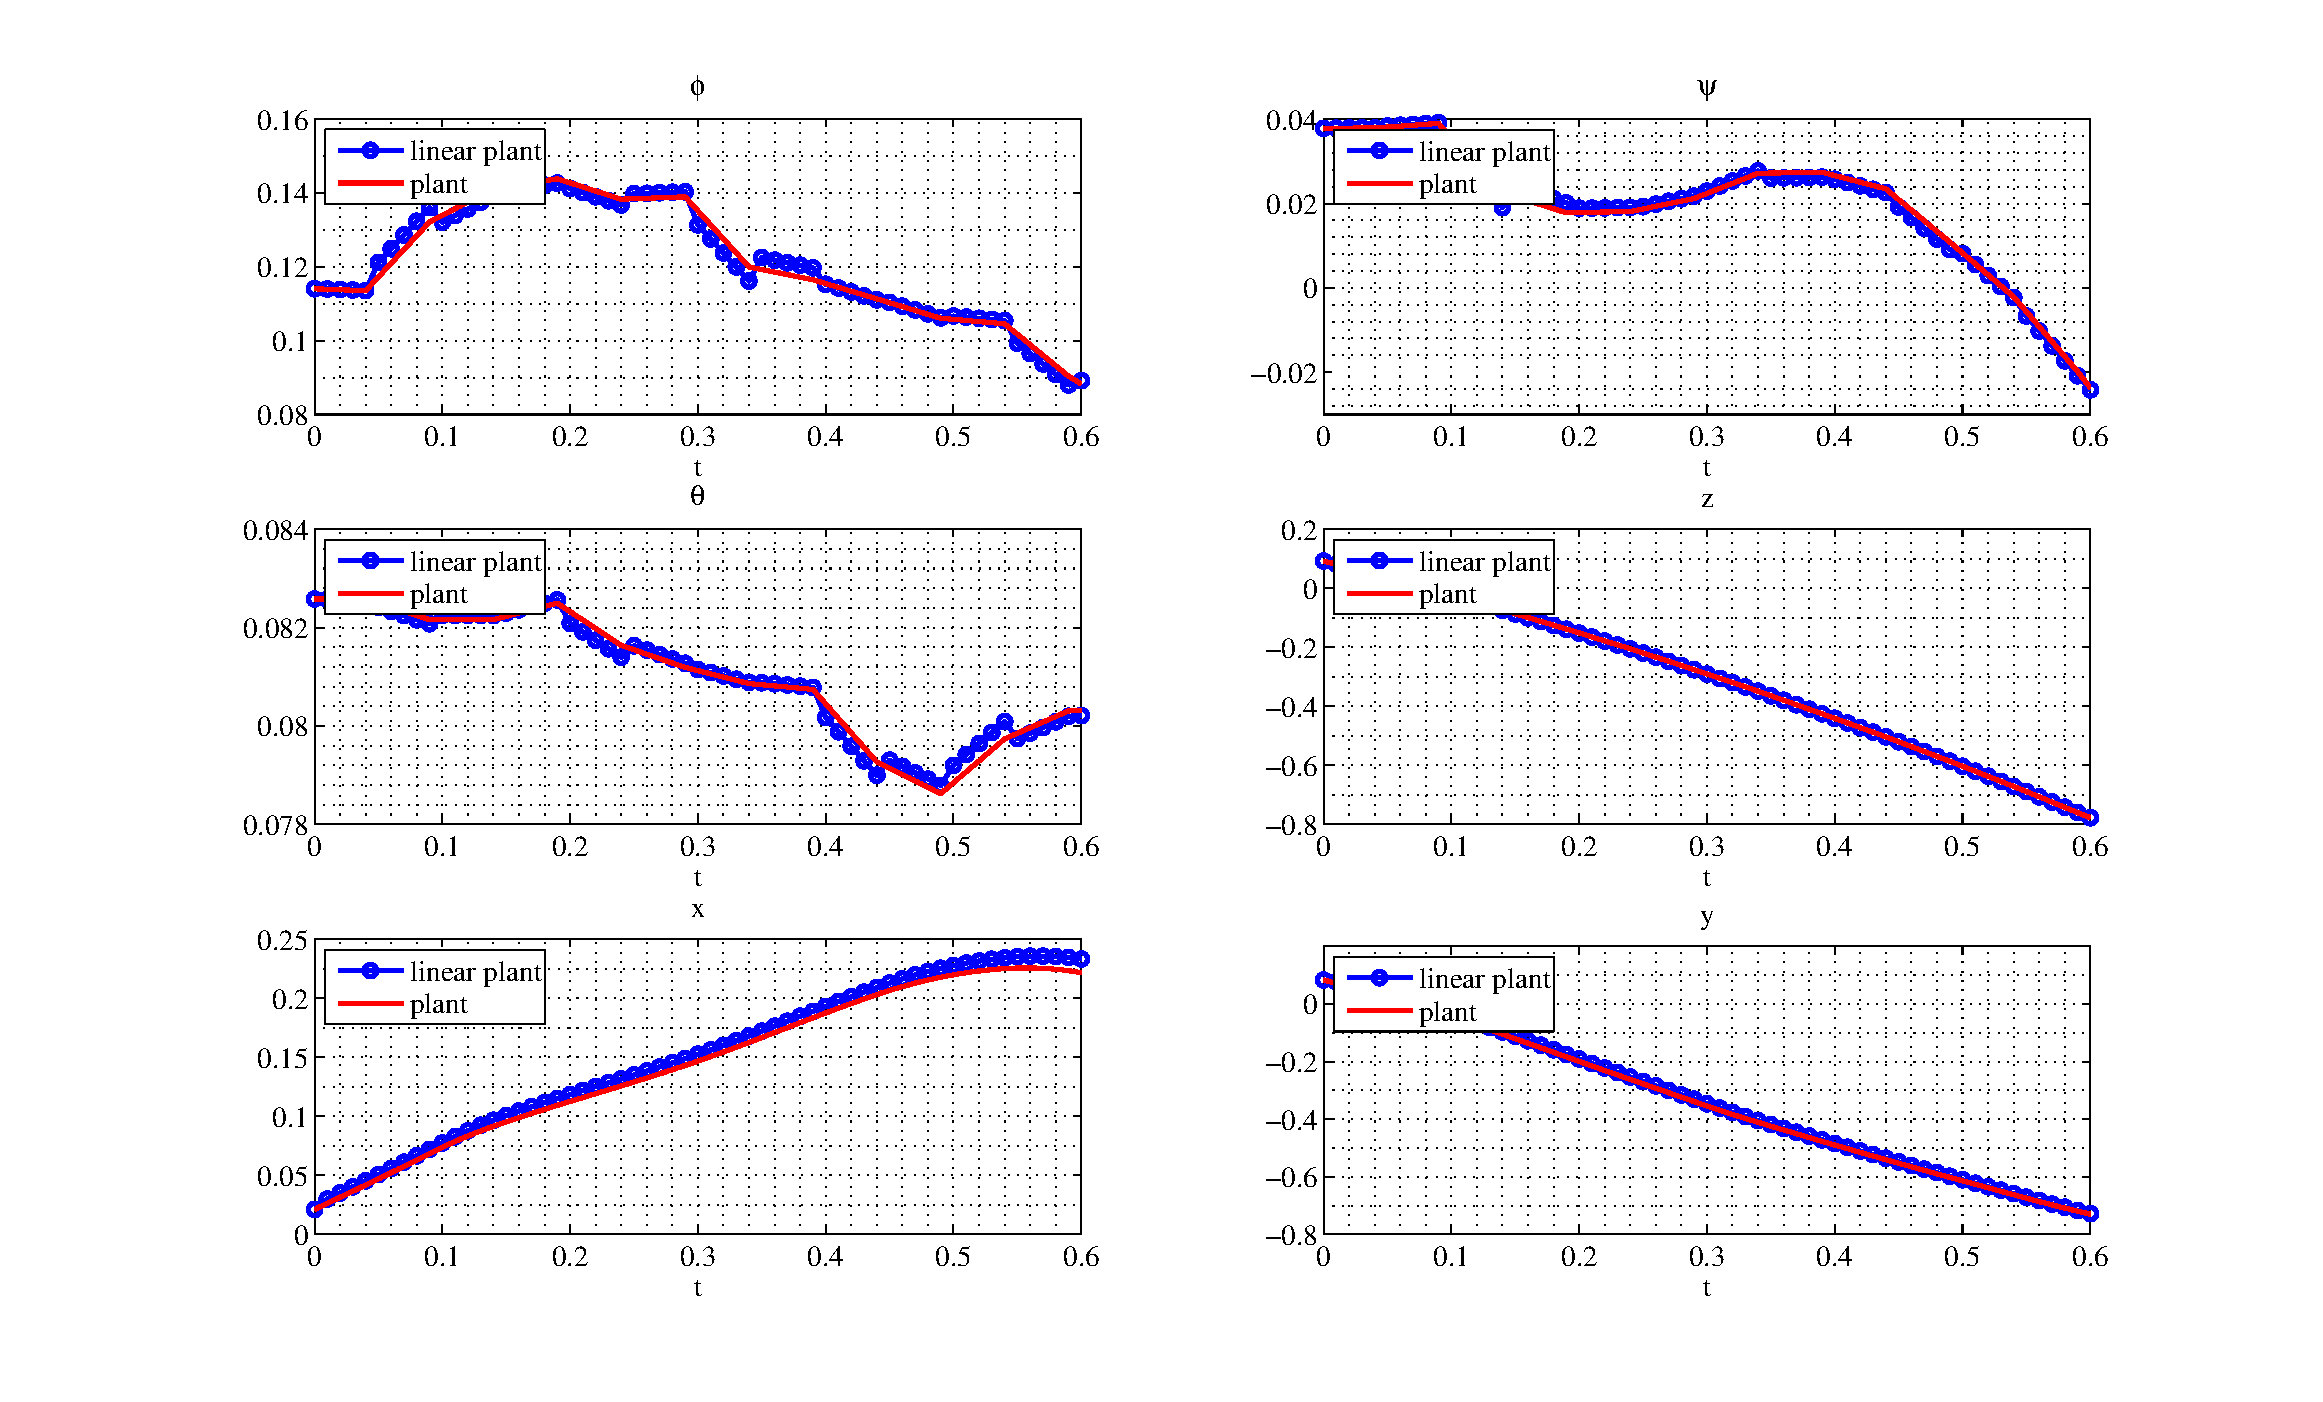
\includegraphics[width=20cm]{linearization.eps}
\caption{Behavior of linearized equations of motion with respect to non-linear equations}
\label{fig:linearization}
\end{figure}

The very limited time-step of $\Delta t = 0.01s$ did not allow us to complete a full simulation of the quadcopter's tracking the path provided by RRT using the full non-linear plant. However, to demonstrate that the MPC does provide satisfactory controls for these very non-linear equations, we used MPC to do a simple reference tracking. We start at the point $(x,y,z) = (0,0,0)$ and ask the quadcopter to move to point $(1,1,-1)$. Note that a value of $z=-1$ is equivalent to climbing $1$ meter. The results of this simulation are presented in Figure \eqref{fig:line_tracking}. We notice that the linearization of the equations provide a very satisfactory result. The weight on the reference error is $10$ and on the changes in control $\delta U$ is $0.005$. The change in control was limited to a magnitude of $1,000$. Because of time-constraints, we were not able to test a more sophisticated cost function.

What is remarkable in these results is that it was indeed possible to let MPC select direct control inputs to the quadcopter's motors and it was not necessary to impose any constraints on the quadcopter's attitude. The proper linearization of the equations was sufficient to allow the MPC algorithm to exploit the coupling between the attitude and the displacements to find a useful solution.

\begin{figure}[]
\centering
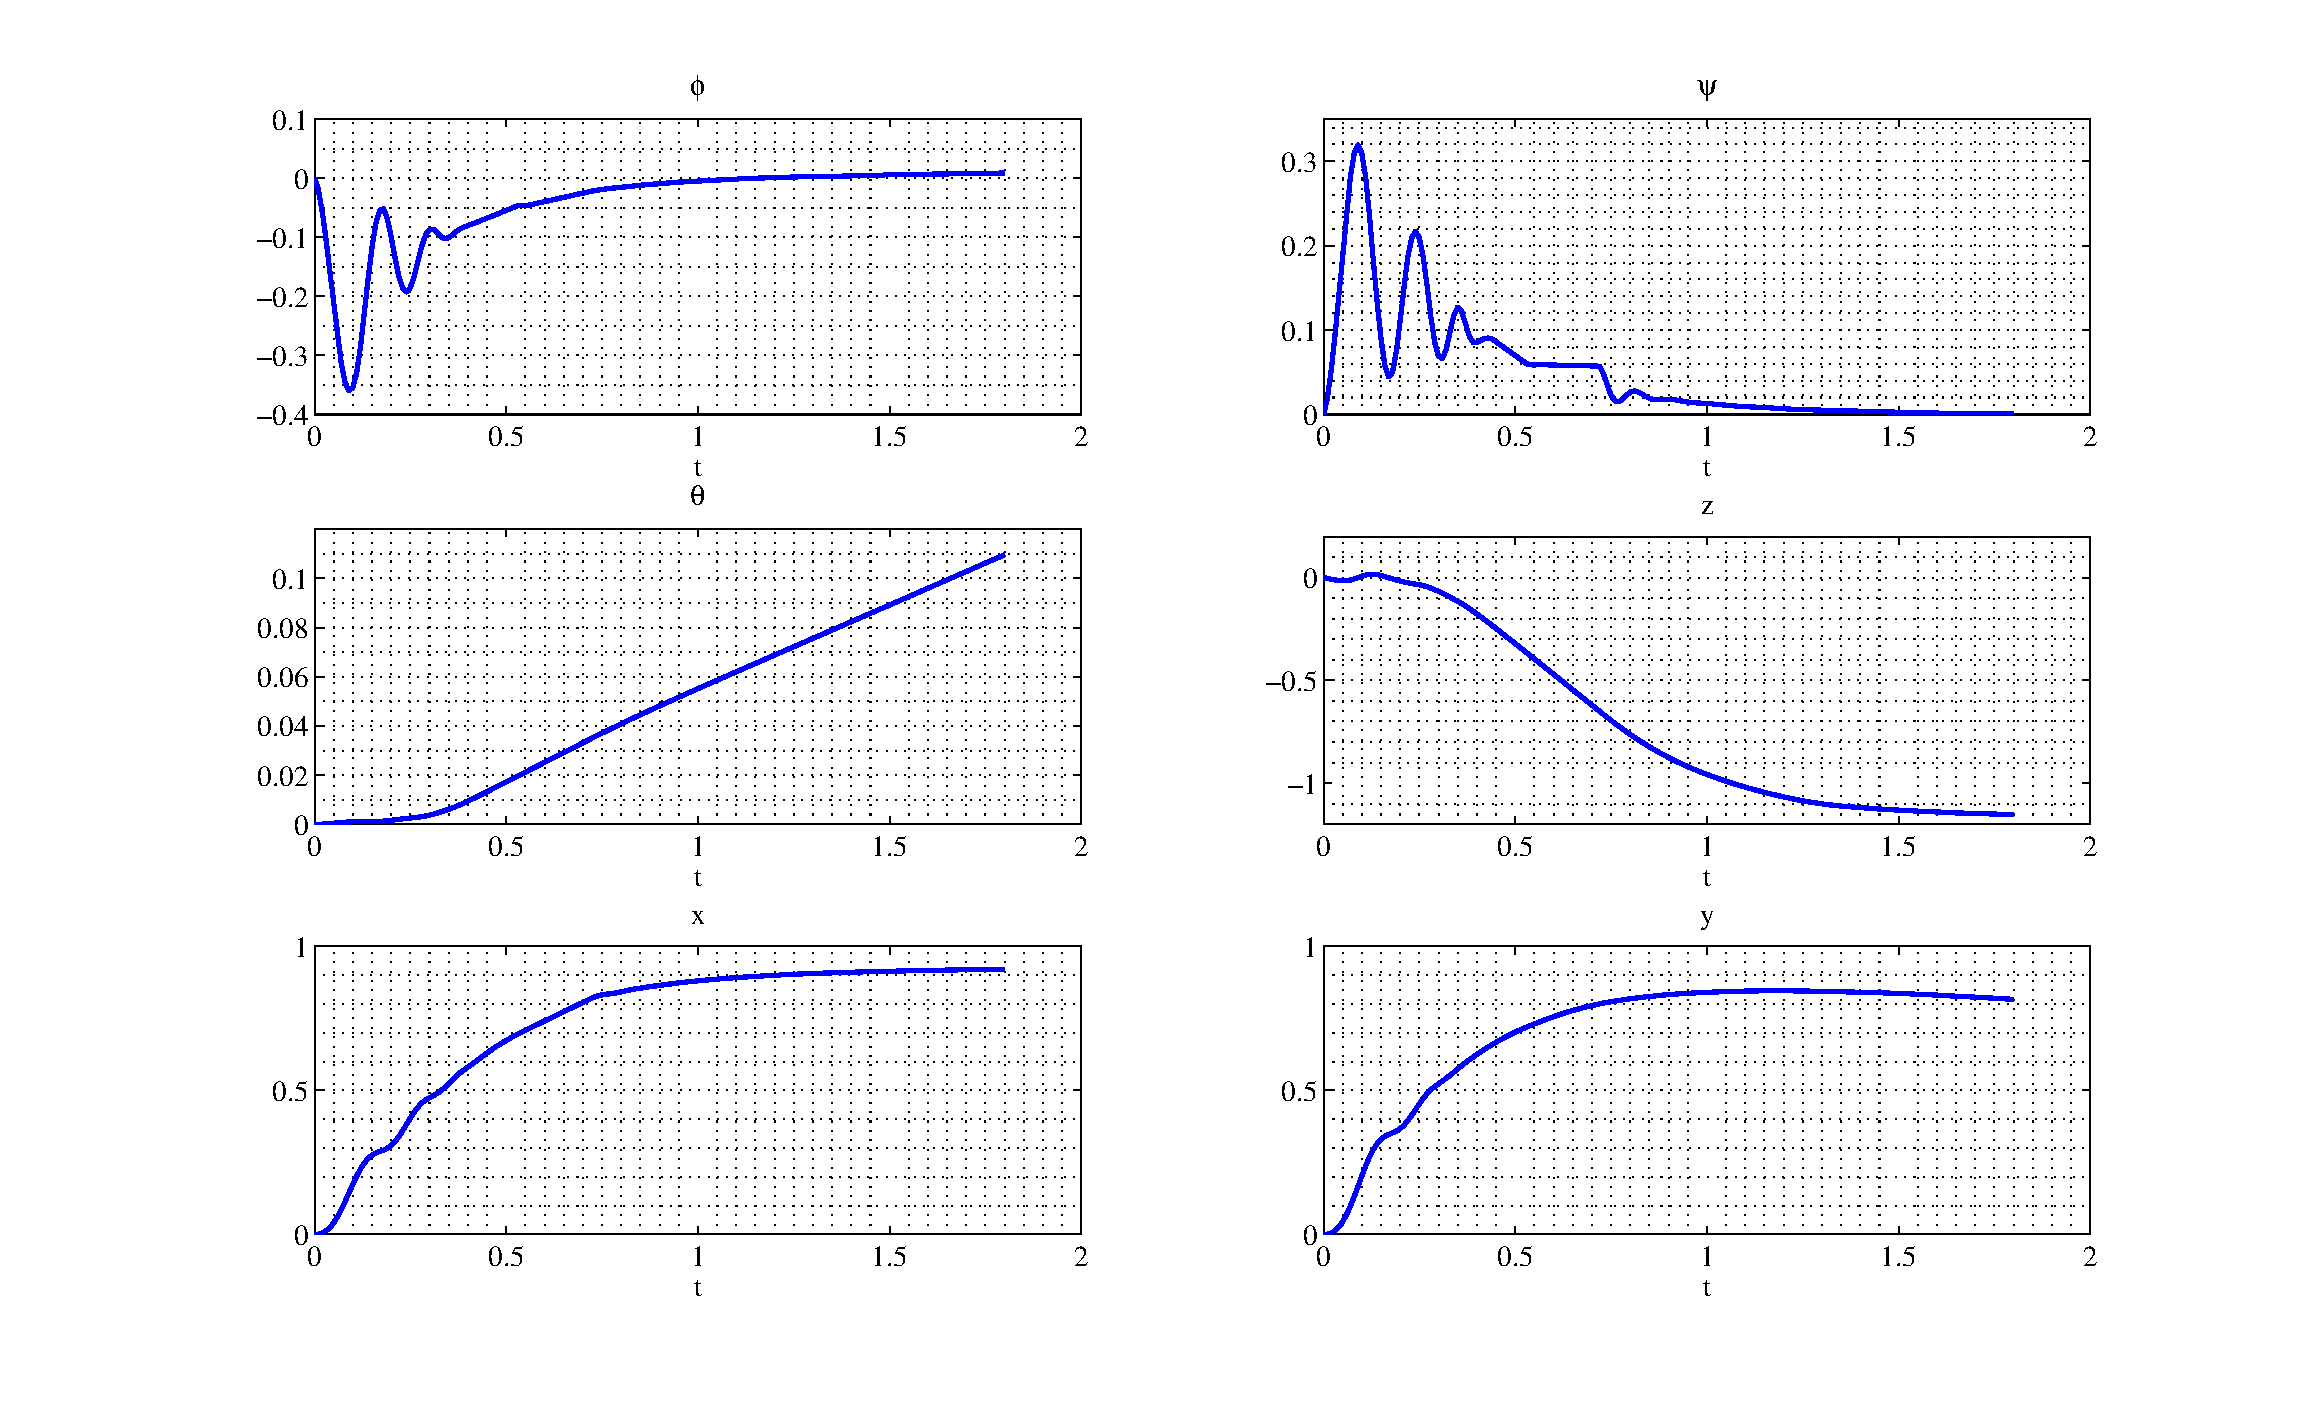
\includegraphics[width=20cm]{line_tracking.eps}
\caption{Attitude and displacement history of a quadcopter moving from $(x,y,z) = (0,0,0)$ to $(1,1,-1)$ using MPC}
\label{fig:line_tracking}
\end{figure}

In order to show that it is possible to get satisfactory results from coupling the MPC algorithm with RRT, we performed simulations on a simplified model of a quadcopter as described in \ref{sub:mpc_simple}. To effectively demonstrate the value of MPC versus an open-loop optimization of inputs, additional components were added to the simulation dynamics.  Random Gaussian noise was added into the position input of the MPC to simulate GPS measurement uncertainty.  A randomly changing disturbance was added to the input vector to simulate windy conditions.  Also, Nonlinear aerodynamic drag was added to the equations of motion. Without a closed-loop control, these effects could not be compensated for.

Videos of the complete simulations for the simplified model are attached. In these videos, the UAV follows the path provided by the RRT until it encounters a new obstacle, at which time a new path is generated and tracked. A picture of one such simulations is in Figure \eqref{fig:sample_simulation}.

\begin{figure}[]
\centering
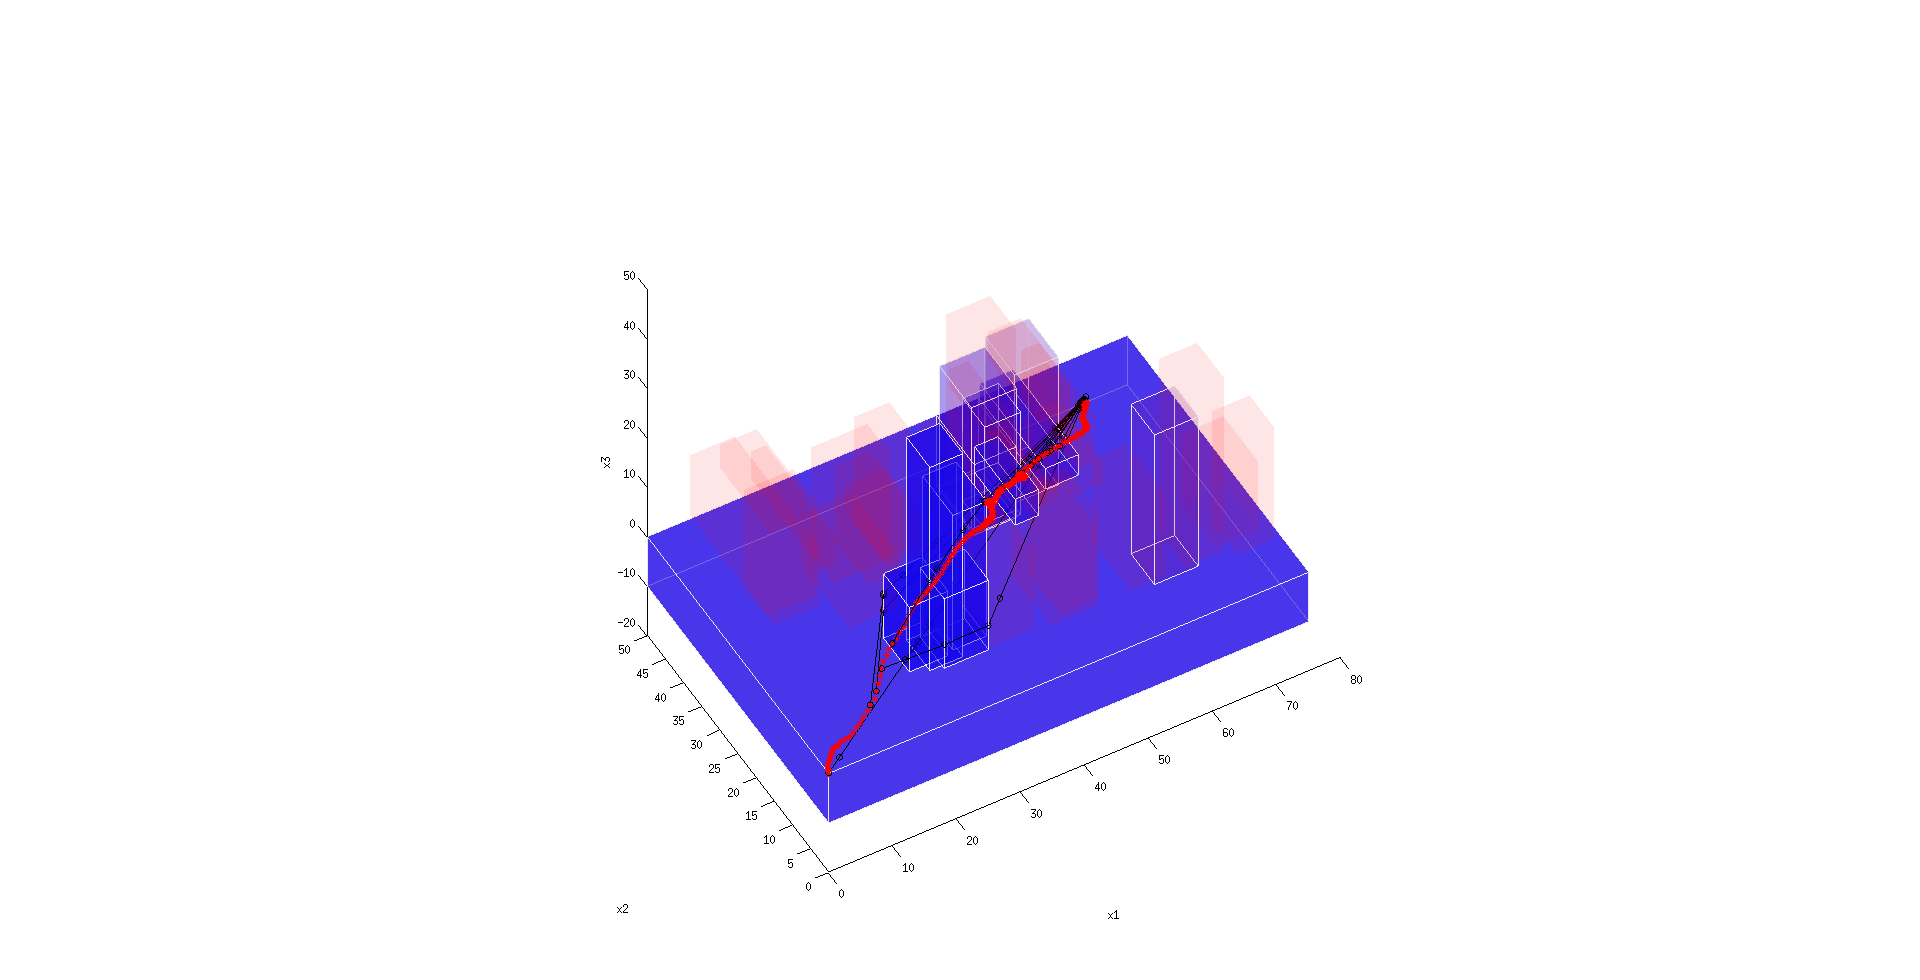
\includegraphics[width=22cm]{sample_simulation.png}
\caption{Picture of a completed simulation run with simplified dynamics. Disturbance forces, sensor uncertainty, and second order drag force are included in this simulation. MPC provides the controls for tracking the line. In blue are the observed obstacles, in red are the unobserved but existing obstacles. The path to track is in black. The quadcopter's center of mass is in red.}
\label{fig:sample_simulation}
\end{figure}


The RRT algorithm worked flawlessly in always finding a path from the arbitrary origin to the arbitrary goal. In the attached videos, unobserved obstacles are in red, observed obstacles are in blue. The darker the blue, the longer time the quadcopter has been aware about the obstacle.